\RequirePackage{amsthm} %https://tex.stackexchange.com/questions/687324/unknown-theoremstyle-warning-with-springer-nature-template
\documentclass[sn-mathphys-num,iicol]{sn-jnl}

%\usepackage{sn-jnl.sty}
\usepackage{graphicx}%
\usepackage{multirow}%
\usepackage{amsmath,amssymb,amsfonts}%
\usepackage{amsthm}%
\usepackage{physics}
\usepackage[locale=DE]{siunitx}
\usepackage{mathrsfs}%
\usepackage[title]{appendix}%
\usepackage{xcolor}%
\usepackage{textcomp}%
\usepackage{manyfoot}%
\usepackage{booktabs}%
\usepackage{algorithm}%
\usepackage{algorithmicx}%
\usepackage{algpseudocode}%
\usepackage{listings}%
\usepackage{newtxmath}%
\usepackage[tiny]{titlesec}%
\usepackage[ngerman]{babel}
\usepackage{booktabs}

\theoremstyle{thmstyleone}
\newtheorem{theorem}{Theorem}
\newtheorem{proposition}[theorem]{Proposition}

\theoremstyle{thmstyletwo}
\newtheorem{remark}{Remark}

\theoremstyle{thmstylethree}
\newtheorem{definition}{Definition}

\raggedbottom

\newcommand{\td}{\text{d}}

\titleformat{\subsection}{}{\thesubsection}{1em}{\itshape}
\titleformat{\subsubsection}{}{\thesubsubsection}{1em}{\itshape}

\begin{document}

\title[]{Praktikum 4 -- Versuch 425: Elektronisches Rauschen}
\author*[1]{\fnm{Jonas} \sur{Wortmann}}\email{s02jwort@uni-bonn.de}
\author*[1]{\fnm{Angelo} \sur{Brade}}\email{s72abrad@uni-bonn.de}
\affil*[1]{Rheinische Friedrich--Wilhelms--Universität, Bonn}

\maketitle

\section{Einleitung}
In jedem elektrischen Schaltkreis ist ein elektronisches Rauschen vorhanden.
Dieses Rauschen setzt sich aus dem \textsc{Johnson}--Rauschen und dem Schrotrauschen zusammen. % TODO: Eigentlich noch aus anderen Rauschen, wie dem des Verstärkers
Das \textsc{Johnson}--Rauschen ist temperaturabhängig, daraus lässt sich die \textsc{Boltzmann}--Konstante bestimmen.
Das Schrotrauschen wird durch die Quantelung der Elementarladung hervorgerufen.
Die Größe der Elementarladung lässt sich damit bestimmen.

\section{Bandbreite}
\subsection{Theoretischer Hintergrund}
\footnote{Die Abweichung der Messwerte von der Literatur wird immer in $[\cdot ]$ hinter dem Messwert angegeben.}Die Bandbreite gibt die Breite eines Frequenzsbands an.
Da das elektronische Rauschen von der Bandbreite abhängig ist, wird diese mit einem Bandpass vorgegeben.
Ein Frequenzband einer bestimmten Breite kann mit einem Hoch-- und Tiefpass in Serie (auch Bandpass) erzeugt werden.
Die im Versuch verwendete Anordnung ist in Abb.\ (\ref{fig:schaltplan_bandpass}) gezeigt.

\begin{figure}[t]
	\centering
	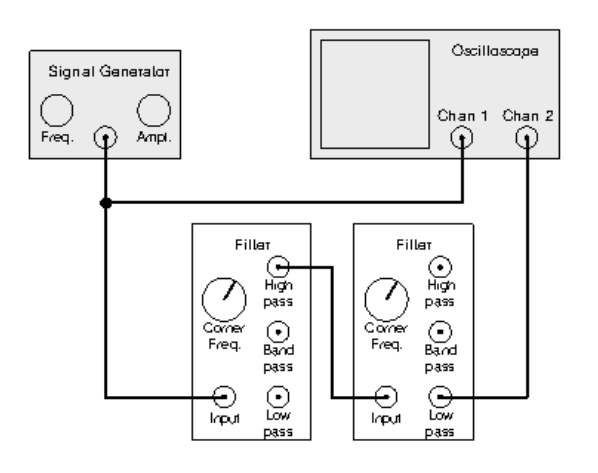
\includegraphics[width=.5\textwidth]{425_schaltplan_bandpass.png}
	\caption{Schaltplan des Bandpass.\cite{anleitung425}} \label{fig:schaltplan_bandpass}
\end{figure}

Die effektive Bandbreite wird mit der Verstärkung
\begin{align}
	G(f)=\dfrac{V^\textsc{rms}_\text{output}}{V^\textsc{rms}_\text{input}}
\end{align}
bestimmt
\begin{align}
	\Delta f_\text{eff}=\int_{0}^{\infty}\td fG^2(f)=\int_{0}^{\infty}\td fG_\text{LP}^2(f)G_\text{HP}^2(f)
	,\end{align}
mit der Tiefpassverstärkung $G_\text{LP}(f)=\left(1+(f/f_\text{l})^4\right)^{-1/2}$ und der Hochpassverstärkung $G_\text{HP}\left(f\right)=\left(f/f_\text{h}\right)^2\left(1+(f/f_\text{h})^4\right)^{-1/2}$.
$f_\text{h}$ und $f_\text{l}$ sind die eingestellten Grenzfrequenzen von Hoch-- und Tiefpass.
Das analytische Ergebnis des Integrals ist
\begin{align}
	\Delta f_\text{eff}=\dfrac{f_\text{l}^4\pi \left(f_\text{h}-f_\text{l}\right)}{2^{3/2}\left(f_\text{h}^4-f_\text{l}^4\right)}
	.\end{align}

\subsection{Durchführung \& Auswertung}
Die Bandbreite wird für $f_\text{h}=\SI{1}{kHz}$ und $f_\text{l}=\SI{10}{kHz}$ bestimmt. % TODO: fh=100Hz fälschlich eigentlich
Mit dem Frequenzgenerator werden, für eine konstante Eingangsspannung, verschiedene Frequenzen von $\SI{2}{Hz}$ bis $\SI{8}{MHz}$ eingestellt und die Ausgangsspannung gemessen.
Daraus bestimmt sich jeweils die Verstärkung und damit die Bandbreite.

Abb.\ (\ref{fig:bandpass}) zeigt die Verstärkung gegen die eingestellte Frequenz.
Die Bandbreite berechnet sich dann zu
\begin{align}
	\Delta f_\text{eff}\approx \SI{9997}{Hz} % TODO: Es gibt noch die Frequenz mit der Anpassung für fl, fh und df
	.\end{align}

\begin{figure}[t]
	\centering
	\resizebox{.5\textwidth}{!}{% GNUPLOT: LaTeX picture with Postscript
\begingroup
  \makeatletter
  \providecommand\color[2][]{%
    \GenericError{(gnuplot) \space\space\space\@spaces}{%
      Package color not loaded in conjunction with
      terminal option `colourtext'%
    }{See the gnuplot documentation for explanation.%
    }{Either use 'blacktext' in gnuplot or load the package
      color.sty in LaTeX.}%
    \renewcommand\color[2][]{}%
  }%
  \providecommand\includegraphics[2][]{%
    \GenericError{(gnuplot) \space\space\space\@spaces}{%
      Package graphicx or graphics not loaded%
    }{See the gnuplot documentation for explanation.%
    }{The gnuplot epslatex terminal needs graphicx.sty or graphics.sty.}%
    \renewcommand\includegraphics[2][]{}%
  }%
  \providecommand\rotatebox[2]{#2}%
  \@ifundefined{ifGPcolor}{%
    \newif\ifGPcolor
    \GPcolortrue
  }{}%
  \@ifundefined{ifGPblacktext}{%
    \newif\ifGPblacktext
    \GPblacktexttrue
  }{}%
  % define a \g@addto@macro without @ in the name:
  \let\gplgaddtomacro\g@addto@macro
  % define empty templates for all commands taking text:
  \gdef\gplbacktext{}%
  \gdef\gplfronttext{}%
  \makeatother
  \ifGPblacktext
    % no textcolor at all
    \def\colorrgb#1{}%
    \def\colorgray#1{}%
  \else
    % gray or color?
    \ifGPcolor
      \def\colorrgb#1{\color[rgb]{#1}}%
      \def\colorgray#1{\color[gray]{#1}}%
      \expandafter\def\csname LTw\endcsname{\color{white}}%
      \expandafter\def\csname LTb\endcsname{\color{black}}%
      \expandafter\def\csname LTa\endcsname{\color{black}}%
      \expandafter\def\csname LT0\endcsname{\color[rgb]{1,0,0}}%
      \expandafter\def\csname LT1\endcsname{\color[rgb]{0,1,0}}%
      \expandafter\def\csname LT2\endcsname{\color[rgb]{0,0,1}}%
      \expandafter\def\csname LT3\endcsname{\color[rgb]{1,0,1}}%
      \expandafter\def\csname LT4\endcsname{\color[rgb]{0,1,1}}%
      \expandafter\def\csname LT5\endcsname{\color[rgb]{1,1,0}}%
      \expandafter\def\csname LT6\endcsname{\color[rgb]{0,0,0}}%
      \expandafter\def\csname LT7\endcsname{\color[rgb]{1,0.3,0}}%
      \expandafter\def\csname LT8\endcsname{\color[rgb]{0.5,0.5,0.5}}%
    \else
      % gray
      \def\colorrgb#1{\color{black}}%
      \def\colorgray#1{\color[gray]{#1}}%
      \expandafter\def\csname LTw\endcsname{\color{white}}%
      \expandafter\def\csname LTb\endcsname{\color{black}}%
      \expandafter\def\csname LTa\endcsname{\color{black}}%
      \expandafter\def\csname LT0\endcsname{\color{black}}%
      \expandafter\def\csname LT1\endcsname{\color{black}}%
      \expandafter\def\csname LT2\endcsname{\color{black}}%
      \expandafter\def\csname LT3\endcsname{\color{black}}%
      \expandafter\def\csname LT4\endcsname{\color{black}}%
      \expandafter\def\csname LT5\endcsname{\color{black}}%
      \expandafter\def\csname LT6\endcsname{\color{black}}%
      \expandafter\def\csname LT7\endcsname{\color{black}}%
      \expandafter\def\csname LT8\endcsname{\color{black}}%
    \fi
  \fi
    \setlength{\unitlength}{0.0500bp}%
    \ifx\gptboxheight\undefined%
      \newlength{\gptboxheight}%
      \newlength{\gptboxwidth}%
      \newsavebox{\gptboxtext}%
    \fi%
    \setlength{\fboxrule}{0.5pt}%
    \setlength{\fboxsep}{1pt}%
    \definecolor{tbcol}{rgb}{1,1,1}%
\begin{picture}(7200.00,4320.00)%
    \gplgaddtomacro\gplbacktext{%
      \csname LTb\endcsname%%
      \put(731,619){\makebox(0,0)[r]{\strut{}$-0.2$}}%
      \csname LTb\endcsname%%
      \put(731,1117){\makebox(0,0)[r]{\strut{}$0$}}%
      \csname LTb\endcsname%%
      \put(731,1615){\makebox(0,0)[r]{\strut{}$0.2$}}%
      \csname LTb\endcsname%%
      \put(731,2113){\makebox(0,0)[r]{\strut{}$0.4$}}%
      \csname LTb\endcsname%%
      \put(731,2611){\makebox(0,0)[r]{\strut{}$0.6$}}%
      \csname LTb\endcsname%%
      \put(731,3110){\makebox(0,0)[r]{\strut{}$0.8$}}%
      \csname LTb\endcsname%%
      \put(731,3608){\makebox(0,0)[r]{\strut{}$1$}}%
      \csname LTb\endcsname%%
      \put(731,4106){\makebox(0,0)[r]{\strut{}$1.2$}}%
      \csname LTb\endcsname%%
      \put(829,425){\makebox(0,0){\strut{}$1$}}%
      \csname LTb\endcsname%%
      \put(1695,425){\makebox(0,0){\strut{}$10$}}%
      \csname LTb\endcsname%%
      \put(2560,425){\makebox(0,0){\strut{}$100$}}%
      \csname LTb\endcsname%%
      \put(3425,425){\makebox(0,0){\strut{}$1000$}}%
      \csname LTb\endcsname%%
      \put(4290,425){\makebox(0,0){\strut{}$10000$}}%
      \csname LTb\endcsname%%
      \put(5155,425){\makebox(0,0){\strut{}$100000$}}%
      \csname LTb\endcsname%%
      \put(6021,425){\makebox(0,0){\strut{}$1\times10^{6}$}}%
      \csname LTb\endcsname%%
      \put(6886,425){\makebox(0,0){\strut{}$1\times10^{7}$}}%
    }%
    \gplgaddtomacro\gplfronttext{%
      \csname LTb\endcsname%%
      \put(170,2362){\rotatebox{-270}{\makebox(0,0){\strut{}$G$}}}%
      \csname LTb\endcsname%%
      \put(3858,135){\makebox(0,0){\strut{}$f/\SI{}{Hz}$}}%
      \csname LTb\endcsname%%
      \put(6123,3932){\makebox(0,0)[r]{\strut{}Hochpass Dominiert}}%
      \csname LTb\endcsname%%
      \put(6123,3738){\makebox(0,0)[r]{\strut{}Tiefpass Dominiert}}%
      \csname LTb\endcsname%%
      \put(6123,3545){\makebox(0,0)[r]{\strut{}Hochpass Modell $G_{\text{HP}}(f)$}}%
      \csname LTb\endcsname%%
      \put(6123,3351){\makebox(0,0)[r]{\strut{}Tiefpass Modell $G_{\text{LP}}(f)$}}%
    }%
    \gplbacktext
    \put(0,0){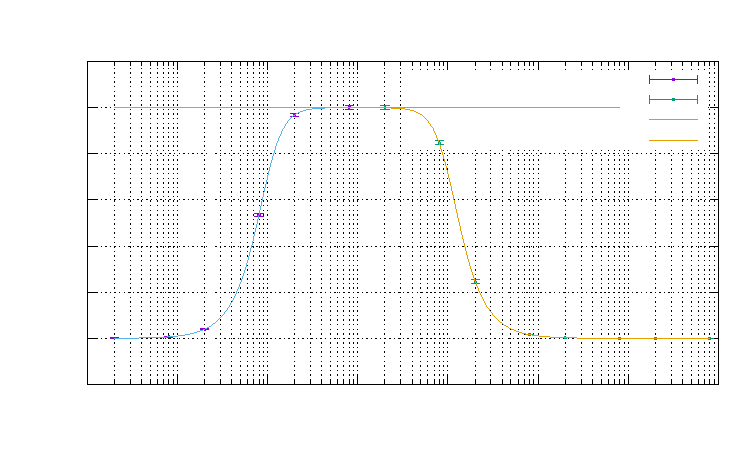
\includegraphics[width={360.00bp},height={216.00bp}]{eff_band}}%
    \gplfronttext
  \end{picture}%
\endgroup
}
	\caption{Gemessene Verstärkung $G=\frac{U_{\text{RMS}}}{U_{0\text{, RMS}}}$ im Bandpass.} \label{fig:bandpass}
\end{figure}

\section{\textsc{Johnson}--Rauschen}
\subsection{Theoretischer Hintergrund}
Das \textsc{Johnson}--Rauschen\footnote{auch thermisches Rauschen} entsteht durch thermodynamische Fluktuationen der Elektronen im Leitungsband.
Dies geschieht, im Vergleich zum Schrotrauschen, ohne, dass eine Spannung angelegt ist.
Elektronen bewegen sich im thermischen Gleichgewicht ungeordnet aufgrund ihrer thermischen Energie wodurch sie kurze Spannungs-- bzw.\ Strompulse erzeugen.
Mit Hilfe von sensitiven Messgeräten kann dieses Rauschen untersucht werden.

Der formale Zusammenhang der mittleren quadratischen Rauschspannung in einem Widerstand $R$ ist
\begin{align}
	\overline{V^2_\text{J}}=4k_\text{B}TR\Delta f_\text{eff}
	,\end{align}
mit der Temperatur $T$ und der Bandbreite $\Delta f_\text{eff}$.

\subsection{Durchführung \& Auswertung: Beobachtung des \textsc{Johnson}--Rauschens}
Das \textsc{Johnson}--Rauschen wird im Vorverstärkerschaltkreis aus Abb.\ (\ref{fig:vorverstärker}) beobachtet.
Diese Schaltung befand sich in der LLE--Box Abb.\ (\ref{fig:johnson_lle}), welche entsprechend verkabelt werden musste.
Zur Beobachtung wurden folgende Werte eingestellt
\begin{align}
	R_\text{in}=\SI{100}{k\ohm},R_\text{f}=\SI{1}{k\ohm}
	.\end{align}
Die LLE--Box wurde dann mit der HLE--Box Abb.\ (\ref{fig:johnson_hle}) verbunden.
Die Einstellung der HLE--Box war
\begin{align}
	f_\text{h}=\SI{.1}{kHz},f_\text{l}=\SI{100}{kHz},\text{Gain}=300,\text{AC}
	.\end{align}
Das Rauschen ließ sich dann auf dem Oszillographen beobachten Abb.\ (\ref{fig:johnson_oszi}).
Es ist klar zu erkennen, dass das Rauschen starken Fluktuationen unterliegt und ungeordnet ist.
Im Mittel bleibt es allerdings konstant.

\begin{figure}[t]
	\centering
	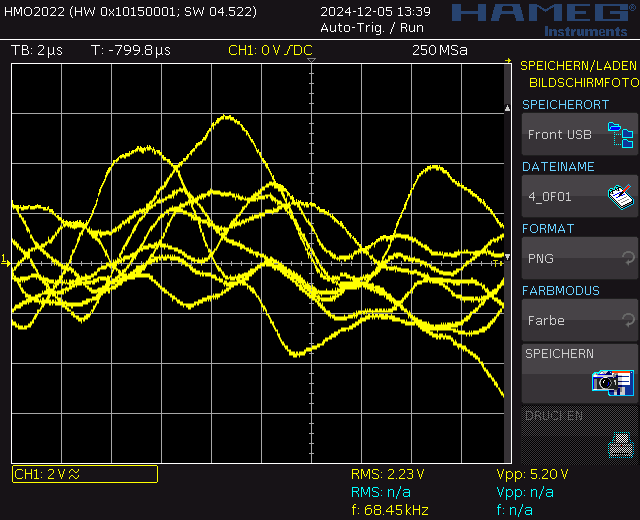
\includegraphics[width=.5\textwidth]{../data/4_0F01.png}
	\caption{Oszillogramm des \textsc{Johnson}--Rauschen.} \label{fig:johnson_oszi}
\end{figure}

\begin{figure}[t]
	\centering
	\includegraphics[width=.5\textwidth]{425_schaltplan_vorverstärker_LLE.png}
	\caption{Vorverstärkerschaltkreis zur Beobachtung des \textsc{Johnson}--Rauschens.\cite{anleitung425}} \label{fig:vorverstärker}
\end{figure}

\begin{figure}[t]
	\centering
	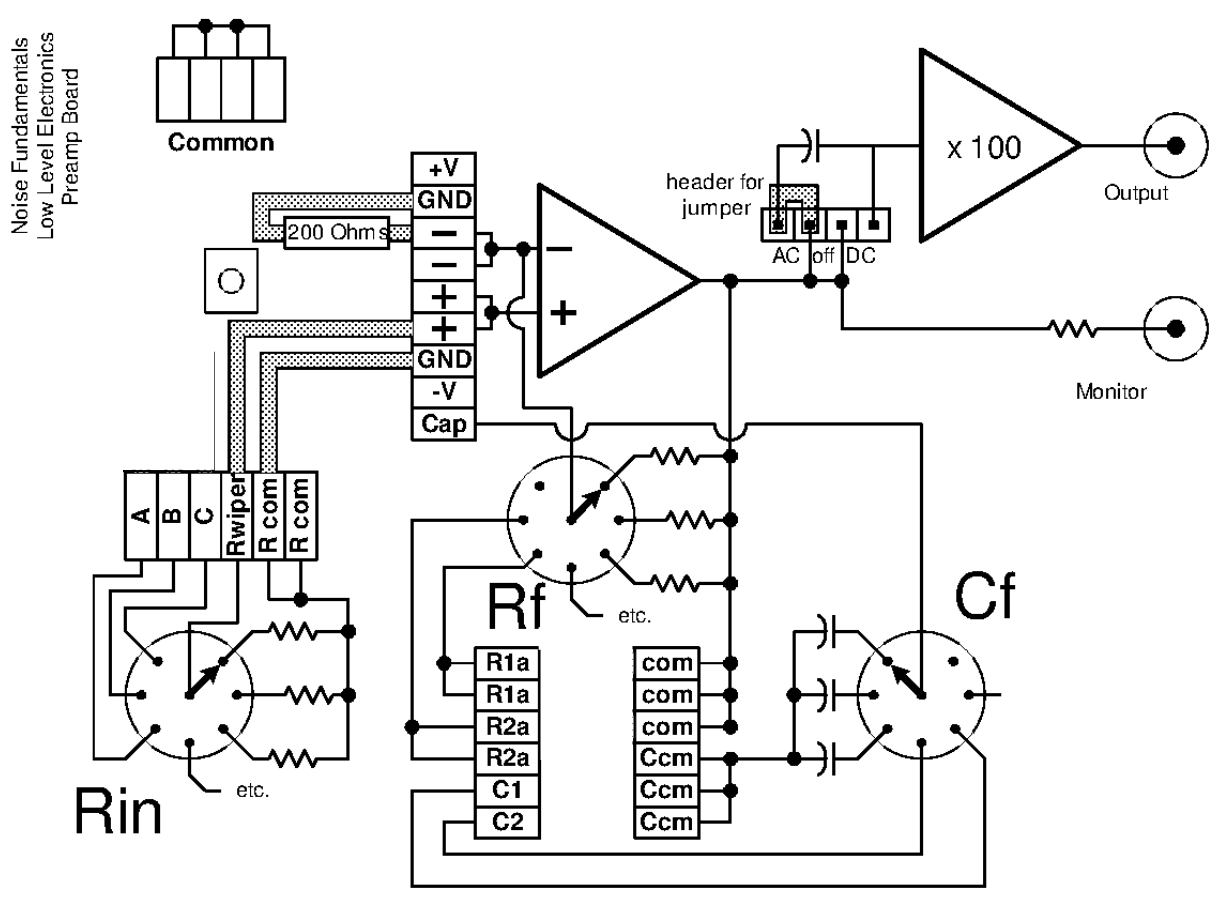
\includegraphics[width=.5\textwidth]{425_schaltplan_johnson_LLE.png}
	\caption{Die LLE--Box zur Messung und Beobachtung des \textsc{Johnson}--Rauschens.\cite{anleitung425}} \label{fig:johnson_lle}
\end{figure}

\begin{figure}[t]
	\centering
	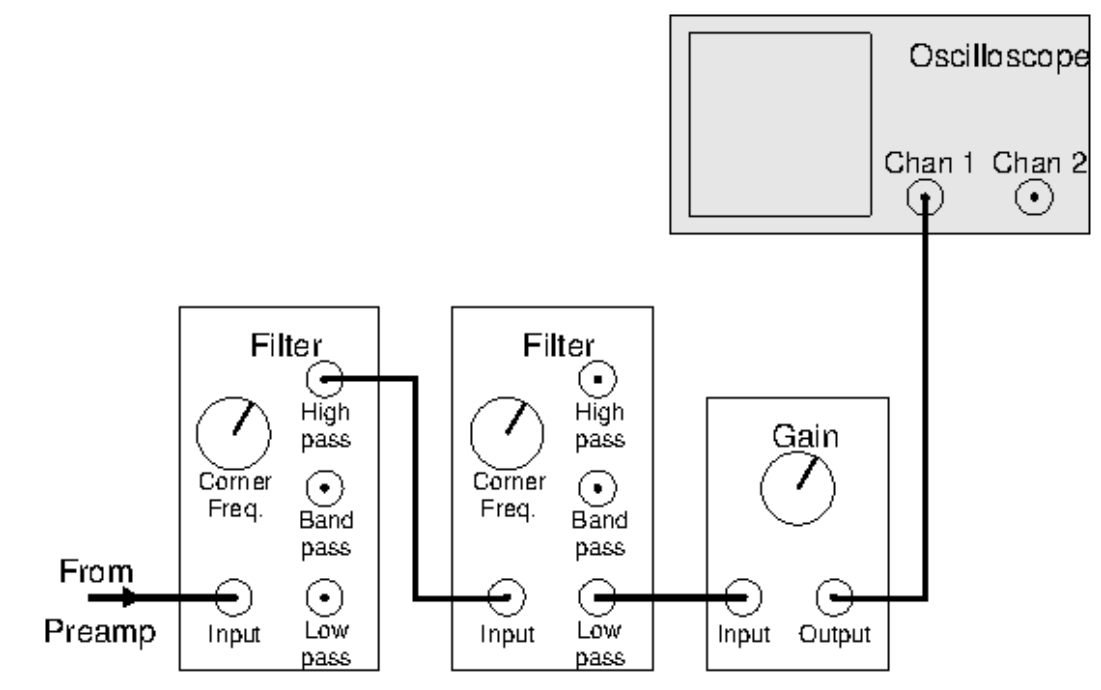
\includegraphics[width=.5\textwidth]{425_schaltplan_visualisierung_johnson_HLE.png}
	\caption{HLE--Box zur Messung und Beobachtung des \textsc{Johnson}--Rauschens.\cite{anleitung425}} \label{fig:johnson_hle}
\end{figure}

\subsection{Durchführung \& Auswertung: Messung des \textsc{Johnson}--Rauschens}
Zur Messung der mittleren Spannung des Rauschens wird die Schaltung aus Abb.\ (\ref{fig:johnson_hle_messung}) verwendet.
Die Einstellungen waren zusätzlich
\begin{align}
	\text{Multiplier}:\text{A}\times \text{A},\text{Zeitkonst.}=\SI{1}{s}
	.\end{align}
Durch den Multiplier ist das Ausgangssignal der HLE--Box
\begin{align}
	V_\text{out}=\dfrac{\overline{\left(V_\text{in}(t)\right)^2}}{\SI{10}{V}}
	.\end{align}
Dieses Signal wird dann über die Zeitkonstante von $\SI{1}{s}$ gemittelt.

Um zu überprüfen, ob der Multiplier wie erwartet funktioniert, kann der Output der HLE--Box gegen den Multiplier aufgetragen werden.
Es ergibt sich Abb.\ (\ref{fig:multiplier}).
Der quadratische Zusammenhang mit Verschiebung ist klar zu erkennen. % TODO: Warum?

Da das Ausgangssignal nur in einem kleinen Bereich -- zwischen $\SI{0.6}{V}$ und $\SI{1.2}{V}$ -- stabil und linear zum Eingangsrauschen ist, wird das DMM mit Hilfe der Verstärkung in diesem Bereich gehalten.
Der Zusammenhang zwischen der am DMM abgelesenen Spannung ist modelliert durch
\begin{align}
	V_\text{meter}=\overline{V_\text{J}^2(t)+V_\text{N}^2(t)}\dfrac{\left(600G_2\right)^2}{\SI{10}{V}}
	,\end{align}
wobei das Rauschen in die beiden Anteile $V_\text{J}$ und $V_\text{N}$ aufgeteilt werden muss.
$V_\text{J}$ ist das \textsc{Johnson}--Rauschen und $V_\text{N}$ ist der Anteil des Rauschens, der innerhalb der Verstärker entsteht.
Eine Korrelation zwischen diesen beiden Rauschtypen gibt es nicht, da sie in unterschiedlichen Bauteilen beobachtet werden. % TODO: Die Erklärung scheint mir etwas zu einfach. Anderes Phänomen, welches nicht Termperaturabhängig ist.
Diese Tatsache erlaubt daher die Bestimmung von $V_\text{J}$ über die Variation des Widerstands $R_\text{in}$, da $V_\text{J}=V_\text{J}(R_\text{in})$ und $V_\text{N}\neq V_\text{N}(R_\text{in})$.
Das \textsc{Johnson}--Rauschen kann zusätzlich über die Variation der Bandbreite erfolgen, da es von der Verstärkung $G_2$ abhängt.

\begin{figure}[t]
	\centering
	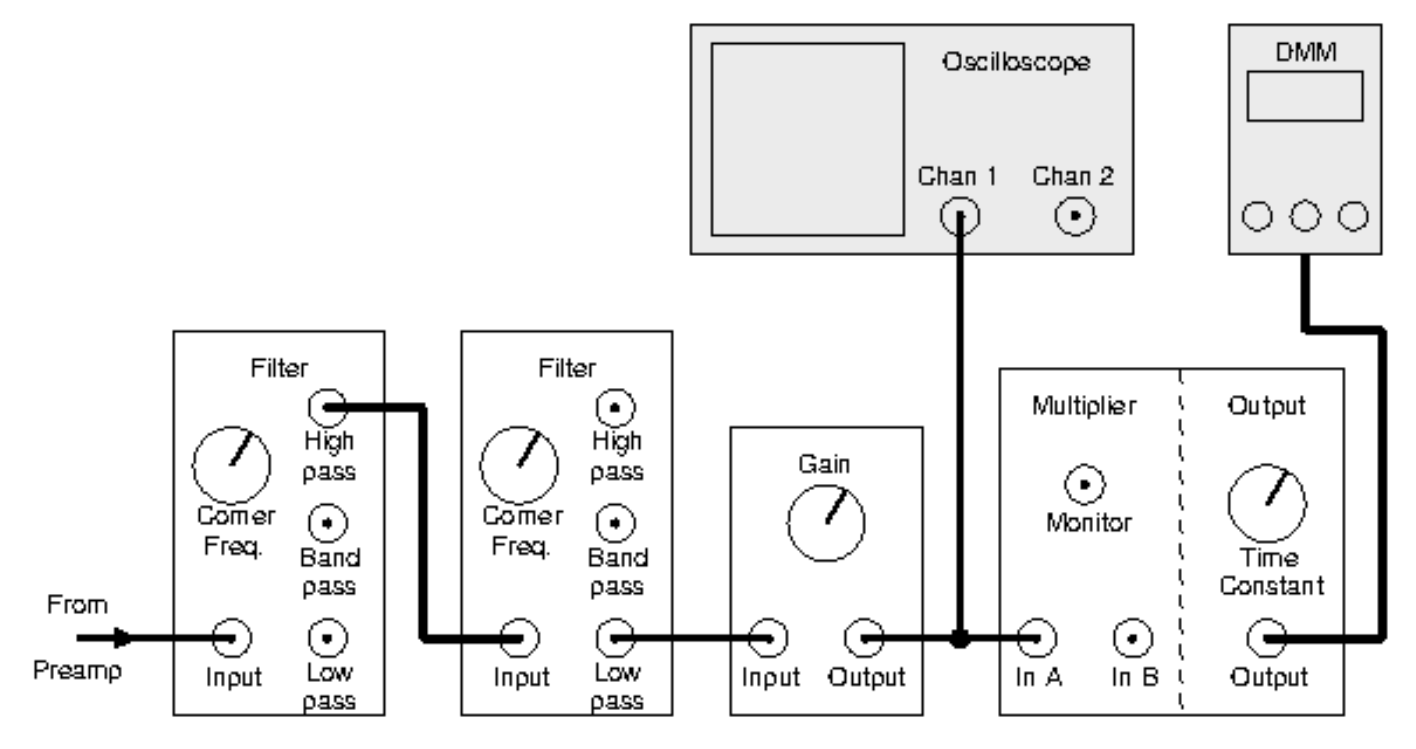
\includegraphics[width=.5\textwidth]{425_schaltplan_messung_johnson.png}
	\caption{HLE--Box zur Messung des \textsc{Johnson}--Rauschens.\cite{anleitung425}} \label{fig:johnson_hle_messung}
\end{figure}

\begin{figure}[t]
	\centering
	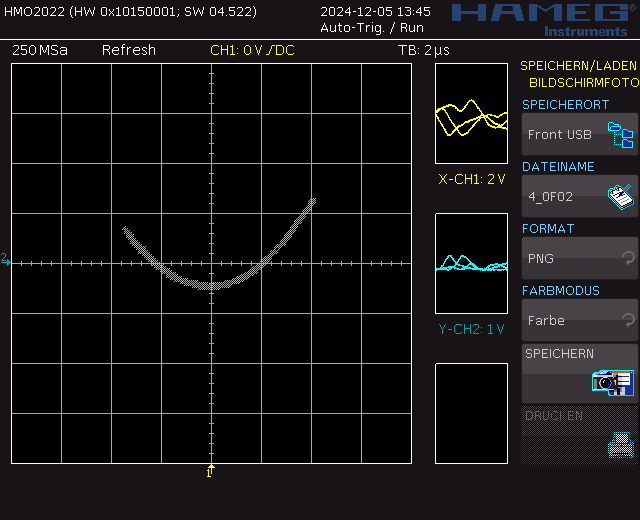
\includegraphics[width=.5\textwidth]{../data/4_0F02.png}
	\caption{Output der HLE--Box (Kanal 1) gegen Multiplier (Kanal 2).} \label{fig:multiplier}
\end{figure}

\subsubsection{Variation des Widerstands}
Wird der Widerstand variiert, um so das \textsc{Johnson}--Rauschen zu bestimmen, ergeben sich Abb.\ (\ref{fig:johnson_widerstand_messung}) mit Tab.\ (\ref{tab:johnson_widerstand_parameter}).

\begin{figure}[t]
	\centering
	\resizebox{.5\textwidth}{!}{\input{Widerstandsabhängigkeit.tex}}
	\caption{Widerstandsabhängigkeit mit $\overline{V_J^2(t)+V_N^2(t)}=V_{\text{meter}}\frac{\SI{10}{V}}{(600\cdot G_2)^2}$} \label{fig:johnson_widerstand_messung}
\end{figure}
\begin{table}[t]
	\centering
	\begin{tabular}{cc}
		\textbf{Parameter} & {\textbf{Wert(Fehler)}}  \\
		\hline
		m                  & \SI{1.51 \pm 0.11e-15}{} \\
		b                  & \SI{7.04 \pm 0.29e-12}{} \\
	\end{tabular}
	\label{tab:johnson_widerstand_parameter}
	\caption{Widerstandsabhängigkeit modelliert mit $\overline{V_J^2(t)+V_N^2(t)}(R_\text{in})=m\cdot R+b$}
\end{table}
\begin{figure}[t]
	\centering
	\resizebox{.5\textwidth}{!}{% GNUPLOT: LaTeX picture with Postscript
\begingroup
  \makeatletter
  \providecommand\color[2][]{%
    \GenericError{(gnuplot) \space\space\space\@spaces}{%
      Package color not loaded in conjunction with
      terminal option `colourtext'%
    }{See the gnuplot documentation for explanation.%
    }{Either use 'blacktext' in gnuplot or load the package
      color.sty in LaTeX.}%
    \renewcommand\color[2][]{}%
  }%
  \providecommand\includegraphics[2][]{%
    \GenericError{(gnuplot) \space\space\space\@spaces}{%
      Package graphicx or graphics not loaded%
    }{See the gnuplot documentation for explanation.%
    }{The gnuplot epslatex terminal needs graphicx.sty or graphics.sty.}%
    \renewcommand\includegraphics[2][]{}%
  }%
  \providecommand\rotatebox[2]{#2}%
  \@ifundefined{ifGPcolor}{%
    \newif\ifGPcolor
    \GPcolortrue
  }{}%
  \@ifundefined{ifGPblacktext}{%
    \newif\ifGPblacktext
    \GPblacktexttrue
  }{}%
  % define a \g@addto@macro without @ in the name:
  \let\gplgaddtomacro\g@addto@macro
  % define empty templates for all commands taking text:
  \gdef\gplbacktext{}%
  \gdef\gplfronttext{}%
  \makeatother
  \ifGPblacktext
    % no textcolor at all
    \def\colorrgb#1{}%
    \def\colorgray#1{}%
  \else
    % gray or color?
    \ifGPcolor
      \def\colorrgb#1{\color[rgb]{#1}}%
      \def\colorgray#1{\color[gray]{#1}}%
      \expandafter\def\csname LTw\endcsname{\color{white}}%
      \expandafter\def\csname LTb\endcsname{\color{black}}%
      \expandafter\def\csname LTa\endcsname{\color{black}}%
      \expandafter\def\csname LT0\endcsname{\color[rgb]{1,0,0}}%
      \expandafter\def\csname LT1\endcsname{\color[rgb]{0,1,0}}%
      \expandafter\def\csname LT2\endcsname{\color[rgb]{0,0,1}}%
      \expandafter\def\csname LT3\endcsname{\color[rgb]{1,0,1}}%
      \expandafter\def\csname LT4\endcsname{\color[rgb]{0,1,1}}%
      \expandafter\def\csname LT5\endcsname{\color[rgb]{1,1,0}}%
      \expandafter\def\csname LT6\endcsname{\color[rgb]{0,0,0}}%
      \expandafter\def\csname LT7\endcsname{\color[rgb]{1,0.3,0}}%
      \expandafter\def\csname LT8\endcsname{\color[rgb]{0.5,0.5,0.5}}%
    \else
      % gray
      \def\colorrgb#1{\color{black}}%
      \def\colorgray#1{\color[gray]{#1}}%
      \expandafter\def\csname LTw\endcsname{\color{white}}%
      \expandafter\def\csname LTb\endcsname{\color{black}}%
      \expandafter\def\csname LTa\endcsname{\color{black}}%
      \expandafter\def\csname LT0\endcsname{\color{black}}%
      \expandafter\def\csname LT1\endcsname{\color{black}}%
      \expandafter\def\csname LT2\endcsname{\color{black}}%
      \expandafter\def\csname LT3\endcsname{\color{black}}%
      \expandafter\def\csname LT4\endcsname{\color{black}}%
      \expandafter\def\csname LT5\endcsname{\color{black}}%
      \expandafter\def\csname LT6\endcsname{\color{black}}%
      \expandafter\def\csname LT7\endcsname{\color{black}}%
      \expandafter\def\csname LT8\endcsname{\color{black}}%
    \fi
  \fi
    \setlength{\unitlength}{0.0500bp}%
    \ifx\gptboxheight\undefined%
      \newlength{\gptboxheight}%
      \newlength{\gptboxwidth}%
      \newsavebox{\gptboxtext}%
    \fi%
    \setlength{\fboxrule}{0.5pt}%
    \setlength{\fboxsep}{1pt}%
    \definecolor{tbcol}{rgb}{1,1,1}%
\begin{picture}(7200.00,4320.00)%
    \gplgaddtomacro\gplbacktext{%
      \csname LTb\endcsname%%
      \put(634,619){\makebox(0,0)[r]{\strut{}$-50$}}%
      \csname LTb\endcsname%%
      \put(634,1117){\makebox(0,0)[r]{\strut{}$0$}}%
      \csname LTb\endcsname%%
      \put(634,1615){\makebox(0,0)[r]{\strut{}$50$}}%
      \csname LTb\endcsname%%
      \put(634,2113){\makebox(0,0)[r]{\strut{}$100$}}%
      \csname LTb\endcsname%%
      \put(634,2611){\makebox(0,0)[r]{\strut{}$150$}}%
      \csname LTb\endcsname%%
      \put(634,3110){\makebox(0,0)[r]{\strut{}$200$}}%
      \csname LTb\endcsname%%
      \put(634,3608){\makebox(0,0)[r]{\strut{}$250$}}%
      \csname LTb\endcsname%%
      \put(634,4106){\makebox(0,0)[r]{\strut{}$300$}}%
      \csname LTb\endcsname%%
      \put(731,425){\makebox(0,0){\strut{}$1$}}%
      \csname LTb\endcsname%%
      \put(1757,425){\makebox(0,0){\strut{}$10$}}%
      \csname LTb\endcsname%%
      \put(2783,425){\makebox(0,0){\strut{}$100$}}%
      \csname LTb\endcsname%%
      \put(3809,425){\makebox(0,0){\strut{}$1000$}}%
      \csname LTb\endcsname%%
      \put(4834,425){\makebox(0,0){\strut{}$10000$}}%
      \csname LTb\endcsname%%
      \put(5860,425){\makebox(0,0){\strut{}$100000$}}%
      \csname LTb\endcsname%%
      \put(6886,425){\makebox(0,0){\strut{}$1\times10^{6}$}}%
    }%
    \gplgaddtomacro\gplfronttext{%
      \csname LTb\endcsname%%
      \put(170,2362){\rotatebox{-270}{\makebox(0,0){\strut{}$\text{res}/\SI{}{\micro V^2}$}}}%
      \csname LTb\endcsname%%
      \put(3809,135){\makebox(0,0){\strut{}$R/\SI{}{\Omega}$}}%
      \csname LTb\endcsname%%
      \put(6123,793){\makebox(0,0)[r]{\strut{}Residuen}}%
    }%
    \gplbacktext
    \put(0,0){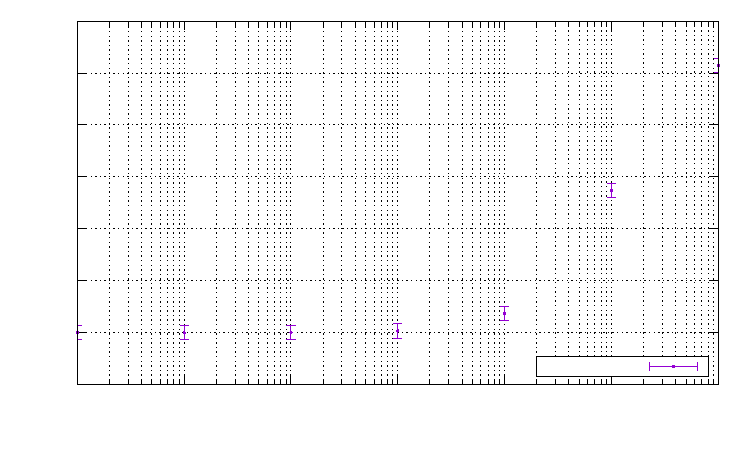
\includegraphics[width={360.00bp},height={216.00bp}]{Widerstandsresiduen}}%
    \gplfronttext
  \end{picture}%
\endgroup
}
	\caption{$\text{res}=\overline{u^2}-\hat{\overline{u^2}}$}
\end{figure}
Es ist
\begin{align}
	\overline{V_\text{J}^2+V_\text{N}^2}=4k_B^RRT\Delta f_\text{eff}+\overline{V_\text{N}^2}
	.\end{align}
Aus der Anpassung geht hervor
\begin{align}
	\overline{V_\text{J}^2+V_\text{N}^2}=mR+b
	,\end{align}
sodass
\begin{align}
	k_B^R=\dfrac{m}{4T\Delta f_\text{eff}}\qquad \overline{V_\text{N}^2}=b
	.\end{align}
Die Temperatur war $T=\SI{252.3+-0.2}{K}$ und die Bandbreite $\Delta f_\text{eff}\approx \SI{11109+-60}{Hz}$.
Damit ist die \textsc{Boltzmann}--Konstante
\begin{align}
	k_B^R          & =\SI{11.53+-0.09e-23}{J/K}[836\%] \\
	k_B^\text{lit} & =\SI{1.380e-23}{J/K}
\end{align}
Der Literaturwert ist entnommen von CODATA\cite{codataBoltzmann}.
DISKUSSION (+ RESIDUEN)

\subsubsection{Variation der Bandbreite}
Dieses Verfahren ist analog zur Variation des Widerstands.
Wird die Bandbreite Variiert, um so das \textsc{Johnson}--Rauschen zu bestimmen, ergeben sich Abb.\ (\ref{fig:johnson_bandbreite_plot}) mit Tab.\ (\ref{tab:johnson_bandbreite_parameter}). % TODO: refs funktionieren nicht

\begin{figure}[h]
	\centering
	\resizebox{.5\textwidth}{!}{% GNUPLOT: LaTeX picture with Postscript
\begingroup
  \makeatletter
  \providecommand\color[2][]{%
    \GenericError{(gnuplot) \space\space\space\@spaces}{%
      Package color not loaded in conjunction with
      terminal option `colourtext'%
    }{See the gnuplot documentation for explanation.%
    }{Either use 'blacktext' in gnuplot or load the package
      color.sty in LaTeX.}%
    \renewcommand\color[2][]{}%
  }%
  \providecommand\includegraphics[2][]{%
    \GenericError{(gnuplot) \space\space\space\@spaces}{%
      Package graphicx or graphics not loaded%
    }{See the gnuplot documentation for explanation.%
    }{The gnuplot epslatex terminal needs graphicx.sty or graphics.sty.}%
    \renewcommand\includegraphics[2][]{}%
  }%
  \providecommand\rotatebox[2]{#2}%
  \@ifundefined{ifGPcolor}{%
    \newif\ifGPcolor
    \GPcolortrue
  }{}%
  \@ifundefined{ifGPblacktext}{%
    \newif\ifGPblacktext
    \GPblacktexttrue
  }{}%
  % define a \g@addto@macro without @ in the name:
  \let\gplgaddtomacro\g@addto@macro
  % define empty templates for all commands taking text:
  \gdef\gplbacktext{}%
  \gdef\gplfronttext{}%
  \makeatother
  \ifGPblacktext
    % no textcolor at all
    \def\colorrgb#1{}%
    \def\colorgray#1{}%
  \else
    % gray or color?
    \ifGPcolor
      \def\colorrgb#1{\color[rgb]{#1}}%
      \def\colorgray#1{\color[gray]{#1}}%
      \expandafter\def\csname LTw\endcsname{\color{white}}%
      \expandafter\def\csname LTb\endcsname{\color{black}}%
      \expandafter\def\csname LTa\endcsname{\color{black}}%
      \expandafter\def\csname LT0\endcsname{\color[rgb]{1,0,0}}%
      \expandafter\def\csname LT1\endcsname{\color[rgb]{0,1,0}}%
      \expandafter\def\csname LT2\endcsname{\color[rgb]{0,0,1}}%
      \expandafter\def\csname LT3\endcsname{\color[rgb]{1,0,1}}%
      \expandafter\def\csname LT4\endcsname{\color[rgb]{0,1,1}}%
      \expandafter\def\csname LT5\endcsname{\color[rgb]{1,1,0}}%
      \expandafter\def\csname LT6\endcsname{\color[rgb]{0,0,0}}%
      \expandafter\def\csname LT7\endcsname{\color[rgb]{1,0.3,0}}%
      \expandafter\def\csname LT8\endcsname{\color[rgb]{0.5,0.5,0.5}}%
    \else
      % gray
      \def\colorrgb#1{\color{black}}%
      \def\colorgray#1{\color[gray]{#1}}%
      \expandafter\def\csname LTw\endcsname{\color{white}}%
      \expandafter\def\csname LTb\endcsname{\color{black}}%
      \expandafter\def\csname LTa\endcsname{\color{black}}%
      \expandafter\def\csname LT0\endcsname{\color{black}}%
      \expandafter\def\csname LT1\endcsname{\color{black}}%
      \expandafter\def\csname LT2\endcsname{\color{black}}%
      \expandafter\def\csname LT3\endcsname{\color{black}}%
      \expandafter\def\csname LT4\endcsname{\color{black}}%
      \expandafter\def\csname LT5\endcsname{\color{black}}%
      \expandafter\def\csname LT6\endcsname{\color{black}}%
      \expandafter\def\csname LT7\endcsname{\color{black}}%
      \expandafter\def\csname LT8\endcsname{\color{black}}%
    \fi
  \fi
    \setlength{\unitlength}{0.0500bp}%
    \ifx\gptboxheight\undefined%
      \newlength{\gptboxheight}%
      \newlength{\gptboxwidth}%
      \newsavebox{\gptboxtext}%
    \fi%
    \setlength{\fboxrule}{0.5pt}%
    \setlength{\fboxsep}{1pt}%
    \definecolor{tbcol}{rgb}{1,1,1}%
\begin{picture}(7200.00,4320.00)%
    \gplgaddtomacro\gplbacktext{%
      \csname LTb\endcsname%%
      \put(731,619){\makebox(0,0)[r]{\strut{}$-0.2$}}%
      \csname LTb\endcsname%%
      \put(731,1117){\makebox(0,0)[r]{\strut{}$0$}}%
      \csname LTb\endcsname%%
      \put(731,1615){\makebox(0,0)[r]{\strut{}$0.2$}}%
      \csname LTb\endcsname%%
      \put(731,2113){\makebox(0,0)[r]{\strut{}$0.4$}}%
      \csname LTb\endcsname%%
      \put(731,2611){\makebox(0,0)[r]{\strut{}$0.6$}}%
      \csname LTb\endcsname%%
      \put(731,3110){\makebox(0,0)[r]{\strut{}$0.8$}}%
      \csname LTb\endcsname%%
      \put(731,3608){\makebox(0,0)[r]{\strut{}$1$}}%
      \csname LTb\endcsname%%
      \put(731,4106){\makebox(0,0)[r]{\strut{}$1.2$}}%
      \csname LTb\endcsname%%
      \put(829,425){\makebox(0,0){\strut{}$1$}}%
      \csname LTb\endcsname%%
      \put(1695,425){\makebox(0,0){\strut{}$10$}}%
      \csname LTb\endcsname%%
      \put(2560,425){\makebox(0,0){\strut{}$100$}}%
      \csname LTb\endcsname%%
      \put(3425,425){\makebox(0,0){\strut{}$1000$}}%
      \csname LTb\endcsname%%
      \put(4290,425){\makebox(0,0){\strut{}$10000$}}%
      \csname LTb\endcsname%%
      \put(5155,425){\makebox(0,0){\strut{}$100000$}}%
      \csname LTb\endcsname%%
      \put(6021,425){\makebox(0,0){\strut{}$1\times10^{6}$}}%
      \csname LTb\endcsname%%
      \put(6886,425){\makebox(0,0){\strut{}$1\times10^{7}$}}%
    }%
    \gplgaddtomacro\gplfronttext{%
      \csname LTb\endcsname%%
      \put(170,2362){\rotatebox{-270}{\makebox(0,0){\strut{}$G$}}}%
      \csname LTb\endcsname%%
      \put(3858,135){\makebox(0,0){\strut{}$f/\SI{}{Hz}$}}%
      \csname LTb\endcsname%%
      \put(6123,3932){\makebox(0,0)[r]{\strut{}Hochpass Dominiert}}%
      \csname LTb\endcsname%%
      \put(6123,3738){\makebox(0,0)[r]{\strut{}Tiefpass Dominiert}}%
      \csname LTb\endcsname%%
      \put(6123,3545){\makebox(0,0)[r]{\strut{}Hochpass Modell $G_{\text{HP}}(f)$}}%
      \csname LTb\endcsname%%
      \put(6123,3351){\makebox(0,0)[r]{\strut{}Tiefpass Modell $G_{\text{LP}}(f)$}}%
    }%
    \gplbacktext
    \put(0,0){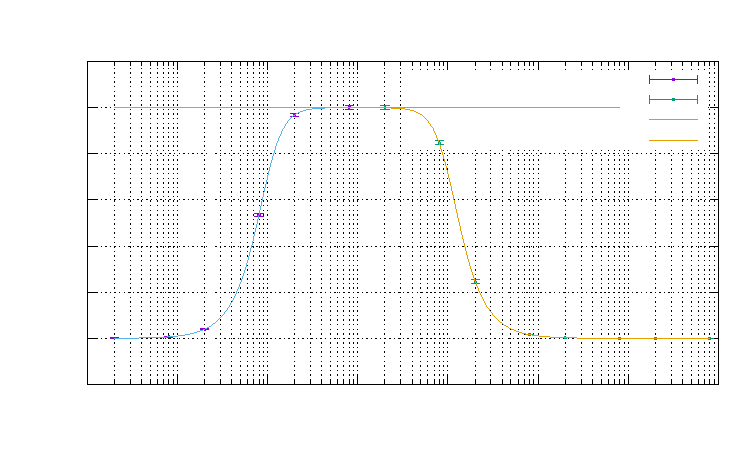
\includegraphics[width={360.00bp},height={216.00bp}]{eff_band}}%
    \gplfronttext
  \end{picture}%
\endgroup
}
	\caption{$G=\frac{U_{\text{RMS}}}{U_{0\text{, RMS}}}$}
\end{figure}
\begin{table}[h!]
	\centering
	\begin{tabular}{cc}
		\textbf{Parameter} & {\textbf{Wert(Fehler)}} \\
		\hline
		$f_l$              & \SI{10104 \pm 56}{}     \\
		$f_h$              & \SI{100.50 \pm 0.17}{}  \\
	\end{tabular}
	\label{tab:parameter}
	\caption{Frequenzabhängigkeit modelliert mit $G_\text{LP}(f)=\left[1+(f/f_l)^4\right]^{-1/2}$ und $G_\text{HP}(f)=(f/f_h)^2\left[1+(f/f_h)^4\right]^{-1/2}$}
\end{table}

\begin{figure}[h]
	\centering
	\resizebox{.5\textwidth}{!}{\input{Bandbreitenabhängigkeit.tex}}
	\caption{Bandbreitenabhängkeit mit $\overline{V_J^2(t)+V_N^2(t)}=V_{\text{meter}}\frac{\SI{10}{V}}{(600\cdot G_2)^2}$ und $\Delta f_{\text{eff}}=\frac{f_l^4\pi (f_l-f_h)}{2^{3/2}(f_l^4-f_h^4)}$}
\end{figure}
\begin{table}[h!]
	\centering
	\begin{tabular}{cc}
		\textbf{Parameter} & {\textbf{Wert(Fehler)}}    \\
		\hline
		m                  & \SI{7.943 \pm 0.069e-17}{} \\
		b                  & \SI{7.5 \pm 4.5e-15}{}     \\
	\end{tabular}
	\label{tab:parameter}
	\caption{Bandbreitenabhängigkeit modelliert mit $\overline{V_J^2(t)+V_N^2(t)}(\Delta f_{\text{eff}})=m\cdot \Delta f_{\text{eff}}+b$}
\end{table}
Es ist
\begin{align}
	\overline{V_\text{J}^2+V_\text{N}^2}=4k_B^fTR_\text{in}\Delta f_\text{eff}+\overline{V_\text{N}^2}
	.\end{align}
Aus der Anpassung geht hervor
\begin{align}
	\overline{V_\text{J}^2+V_\text{N}^2}=m\Delta f_\text{eff}+b
	,\end{align}
sodass
\begin{align}
	k_B^f=\dfrac{m}{4TR_\text{in}}\qquad \overline{V_\text{N}^2}=b
	.\end{align}
Der Widerstand lag bei $R_\text{in}=\SI{1}{k\ohm}$.
Damit ist die \textsc{Boltzmann}--Konstante
\begin{align}
	k_B^f          & =\SI{6.756+-0.06e-23}{J/K}[390\%] \\
	k_B^\text{lit} & =\SI{1.380e-23}{J/K}
\end{align}
Der Literaturwert ist entnommen von CODATA\cite{codataBoltzmann}.
DISKUSSION

\subsubsection{Vergleich Widerstand \& Bandbreite}
Vergleicht man die beiden \textsc{Boltzmann}--Konstanten so liegt die Abweichung bei
\begin{align}
	k_B^R         & =\SI{11.53+-0.09e-23}{J/K}[836\%] \\
	k_B^f         & =\SI{6.756+-0.06e-23}{J/K}[390\%] \\
	|k_B^f-k_B^R| & =\SI{4.774+-0.90e-23}{J/K}        % TODO: Was ist das?
\end{align}
DISKUSSION


\section{Schrotrauschen}
\subsection{Theoretischer Hintergrund}
Da die elektrische Ladung in $e$ gequantelt ist, wird bei dem Übergang von Elektronen über eine Potentialbarriere (z.B.\ zwischen zwei Bauteilen, Photodiode, etc.) stets eine Ladung von genau einem $e$ transferiert.
Da die eingehende Ladung pro Zeit also nicht kontinuierlich ist, kommt es zu nicht stetigen Ausschlägen der Spannung, die über dieses Potential gemessen wird.
Diese Spannung wird als Schrotrauschen auf sensitiven Messgeräten wahrgenommen.

Formal ist das mittlere Rauschstromquadrat
\begin{align}
	\overline{i^2}=2ei_\text{dc}\Delta f_\text{eff}
	,\end{align}
mit $i_\text{dc}$ der angelegten Stromstärke.

\subsection{Durchführung \& Auswertung: Beobachtung des Schrotrauschens}
Das Schrotrauschen wurde innerhalb Abb.\ (\ref{fig:schrot_lle_beob}) bei einer Photodiode beobachtet.
Dafür wurde dieser Schaltkreis in Abb.\ (\ref{fig:schrot_lle_mess}) zusammengesteckt.
Die Elektronen aus der Photodiode wurden von einer Glühlampe herausgelöst, damit diese möglichst unkorreliert sind, um kein gleichmäßiges Rauschen zu erhalten.

Beobachtet wurde der Rauschstrom bzw.\ die Rauschspannung mit Abb.\ (\ref{fig:schaltplan_schrot_mess}).
Damit dies sichtbar war, wurde die Einstellung $f_\text{l}=\SI{100}{kHz}$ für die HLE--Box getroffen. %TODO: Effektive Bandbreite? integral über G_l
Es ergab sich ein ähnliches Bild zum \textsc{Johnson}--Rauschen. %TODO kein bild schrotrauschen beob??

\begin{figure}[t]
	\centering
	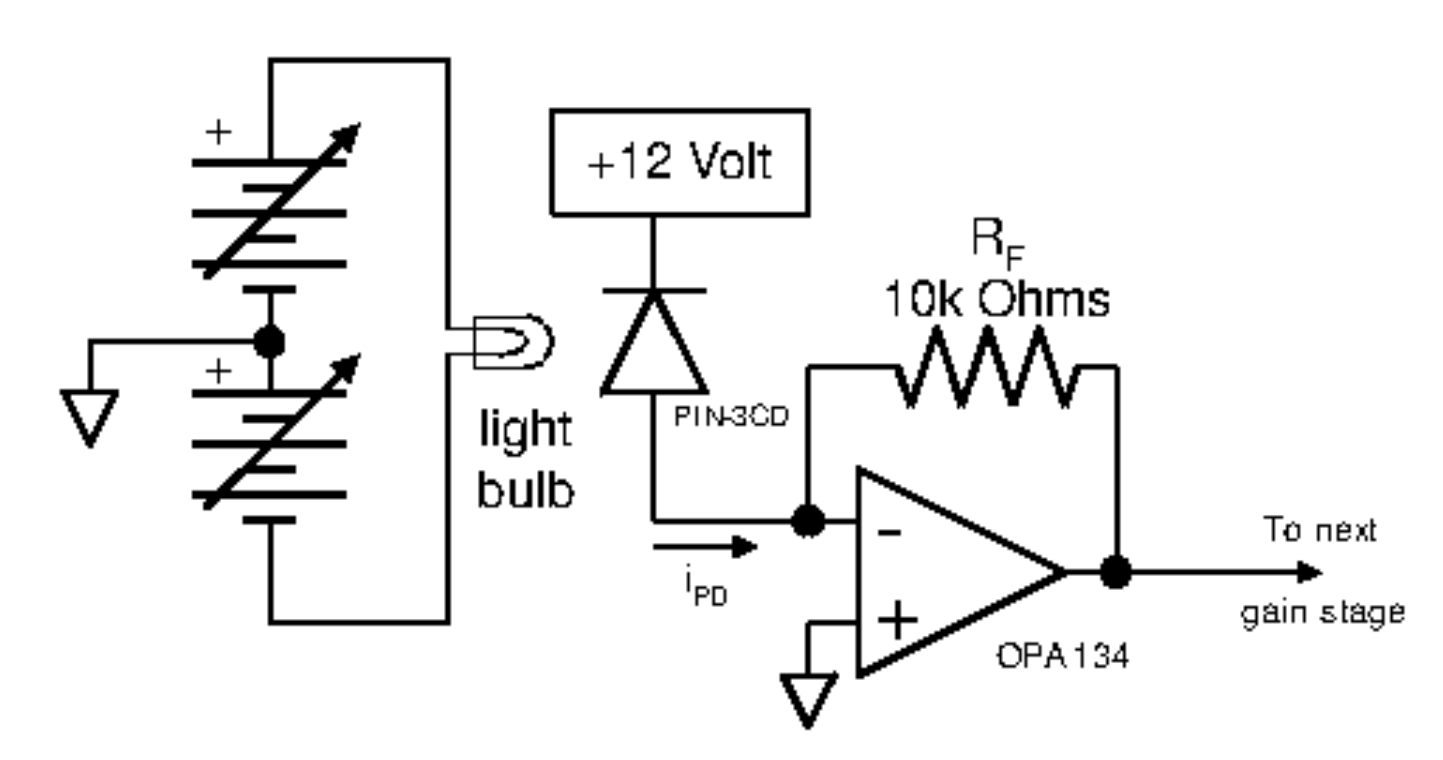
\includegraphics[width=.5\textwidth]{425_schaltplan_visualisierung_schort_LLE.png}
	\caption{Schaltung für die LLE--Box zur Beobachtung und Messung des Schrotrauschens.\cite{anleitung425}} \label{fig:schrot_lle_beob}
\end{figure}
\begin{figure}[t]
	\centering
	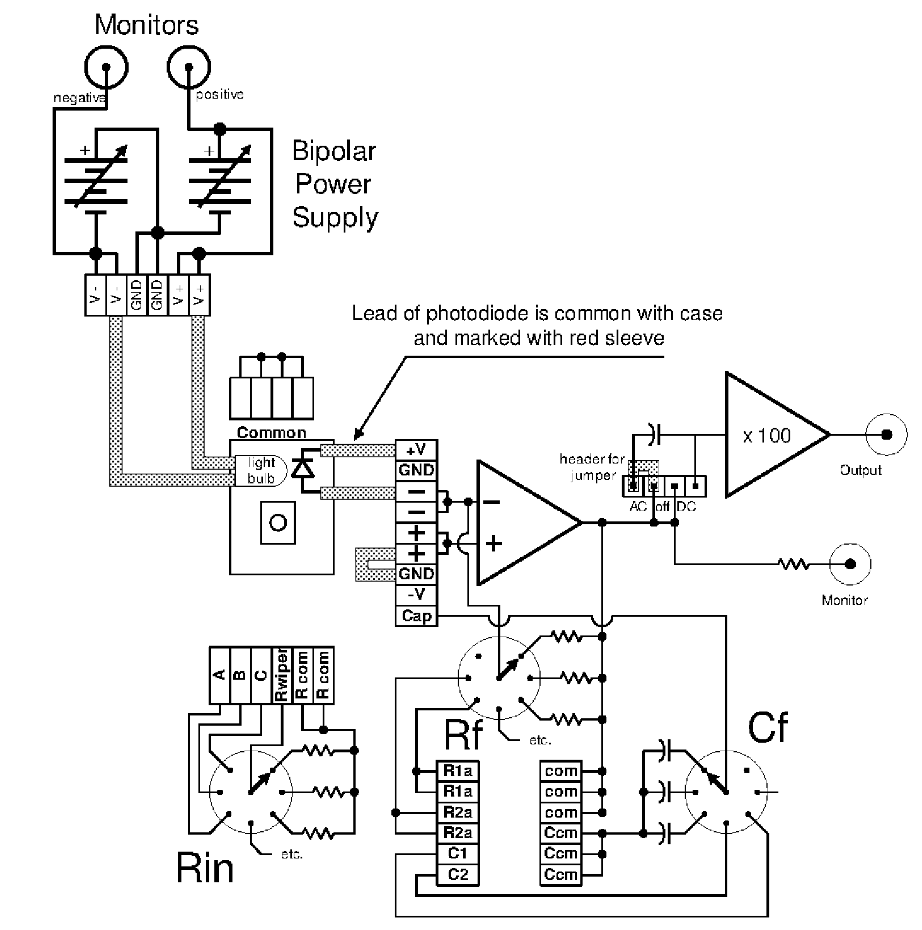
\includegraphics[width=.5\textwidth]{425_schaltplan_messung_schrot_LLE.png}
	\caption{LLE--Box zur Beobachtung und Messung des Schrotrauschens.\cite{anleitung425}} \label{fig:schrot_lle_mess}
\end{figure}
\begin{figure}[t]
	\centering
	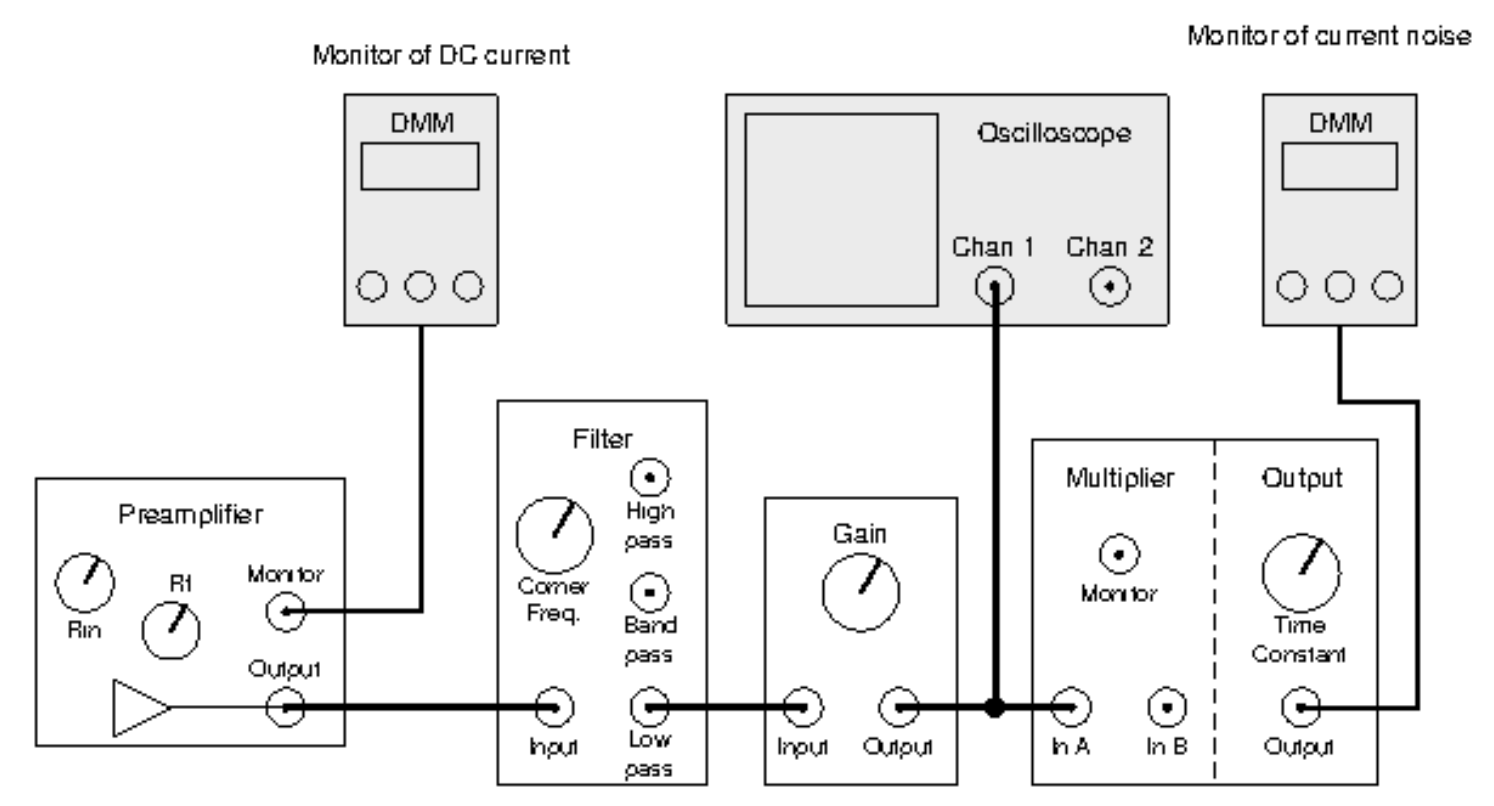
\includegraphics[width=.5\textwidth]{425_schaltplan_messung_schrot.png}
	\caption{Schaltplan zur Messung des Schrotrauschens.\cite{anleitung425}} \label{fig:schaltplan_schrot_mess}
\end{figure}

\subsection{Durchführung \& Auswertung: Messung des Schrotrauschens}
Um den linearen Bereich der Messgeräte zu verwenden, wurde der Gain für jeden Messpunkt so eingestellt, dass die Werte auf dem DMM zwischen $\SI{0.6}{V}$ und $\SI{1.2}{V}$ lagen.
Der Widerstand in der LLE--Box betrug $R_f=\SI{10}{k\ohm}$.
Da der Strom, den der OpAmp zieht, vernachlässigbar klein ist, fließt $i_\text{dc}$ vollständig durch $R_f$, wodurch
\begin{align}
	V_\text{monitor}=-R_fi_\text{dc}
	.\end{align}
Das Schrotrauschen im Schaltkreis war dann gegeben durch
\begin{align}
	\overline{\delta i^2}=\dfrac{\overline{V_\text{meter}(t)}\SI{10}{V}}{(100G_2R_f)^2}
	,\end{align}
mit $\overline{V_\text{meter}(t)}$ dem auf dem DMM abgelesenen Wert und $G_2$ dem Gain der HLE--Box.

\subsubsection{Untergrundbeiträge}
Das gemessene Rauschen entsteht nicht ausschließlich durch das Schrotrauschen.

Das \textsc{Johnson}--Rauschen im $R_f$ Widerstand liefert einen Beitrag.
Um diesen zu berechnen wurde die Ausgabe von $\overline{V_\text{meter}(t)}$ bei ausgeschalteter Lampe gemessen.
Diese liegt bei
\begin{align}
	V_\text{meter}^\text{J}=\SI{1.075+-0.005}{V}\qquad G_2=6000
	.\end{align}
Der Operationsverstärker hat eine gewisse Offset--Spannung bei ausgeschalteter Lampe für $i_\text{dc}=\SI{0}{V}$.
Diese beträgt
\begin{align}
	V_\text{monitor}^\text{OpAmp}=\SI{-0.4+-0.1}{mV} % TODO: Wenn wir hier die Differenz nehmen, bekommmen wir noch den Anteil von dem Bauteil dazwischen
	.\end{align}
Das Aus-- und Einstecken des DMMs ist eine mögliche Quelle für ein weiteres Rauschen, allderdings zeigte dies keinen Effekt an $V_\text{monitor}$.

Diese Beiträge werden in den folgenden Berechnungen berücksichtigt.

\subsubsection{Abhängigkeit $i_\text{dc}$}
Für unterschiedliche Spannungen der Glühlampe stellte sich ein unterschiedlich starkes Rauschen ein, da dieses linear von $i_\text{dc}$ abhängt.
$\overline{\delta i^2}$ gegen $i_\text{dc}$ ist in Abb.\ (\ref{fig:abhängig_idc}) dargestellt.
Die Parameter der Anpassung sind in Tab. (\ref{tab:abhängig_idc_parameter}) eingetragen.
Es ist $R_f=\SI{10}{k\ohm}$.
Der lineare Zusammenhang lässt sich klar erkennen. %TODO chi² oder ist nur guide für auge?

\begin{figure}[t]
	\centering
	\resizebox{.5\textwidth}{!}{% GNUPLOT: LaTeX picture with Postscript
\begingroup
  \makeatletter
  \providecommand\color[2][]{%
    \GenericError{(gnuplot) \space\space\space\@spaces}{%
      Package color not loaded in conjunction with
      terminal option `colourtext'%
    }{See the gnuplot documentation for explanation.%
    }{Either use 'blacktext' in gnuplot or load the package
      color.sty in LaTeX.}%
    \renewcommand\color[2][]{}%
  }%
  \providecommand\includegraphics[2][]{%
    \GenericError{(gnuplot) \space\space\space\@spaces}{%
      Package graphicx or graphics not loaded%
    }{See the gnuplot documentation for explanation.%
    }{The gnuplot epslatex terminal needs graphicx.sty or graphics.sty.}%
    \renewcommand\includegraphics[2][]{}%
  }%
  \providecommand\rotatebox[2]{#2}%
  \@ifundefined{ifGPcolor}{%
    \newif\ifGPcolor
    \GPcolortrue
  }{}%
  \@ifundefined{ifGPblacktext}{%
    \newif\ifGPblacktext
    \GPblacktexttrue
  }{}%
  % define a \g@addto@macro without @ in the name:
  \let\gplgaddtomacro\g@addto@macro
  % define empty templates for all commands taking text:
  \gdef\gplbacktext{}%
  \gdef\gplfronttext{}%
  \makeatother
  \ifGPblacktext
    % no textcolor at all
    \def\colorrgb#1{}%
    \def\colorgray#1{}%
  \else
    % gray or color?
    \ifGPcolor
      \def\colorrgb#1{\color[rgb]{#1}}%
      \def\colorgray#1{\color[gray]{#1}}%
      \expandafter\def\csname LTw\endcsname{\color{white}}%
      \expandafter\def\csname LTb\endcsname{\color{black}}%
      \expandafter\def\csname LTa\endcsname{\color{black}}%
      \expandafter\def\csname LT0\endcsname{\color[rgb]{1,0,0}}%
      \expandafter\def\csname LT1\endcsname{\color[rgb]{0,1,0}}%
      \expandafter\def\csname LT2\endcsname{\color[rgb]{0,0,1}}%
      \expandafter\def\csname LT3\endcsname{\color[rgb]{1,0,1}}%
      \expandafter\def\csname LT4\endcsname{\color[rgb]{0,1,1}}%
      \expandafter\def\csname LT5\endcsname{\color[rgb]{1,1,0}}%
      \expandafter\def\csname LT6\endcsname{\color[rgb]{0,0,0}}%
      \expandafter\def\csname LT7\endcsname{\color[rgb]{1,0.3,0}}%
      \expandafter\def\csname LT8\endcsname{\color[rgb]{0.5,0.5,0.5}}%
    \else
      % gray
      \def\colorrgb#1{\color{black}}%
      \def\colorgray#1{\color[gray]{#1}}%
      \expandafter\def\csname LTw\endcsname{\color{white}}%
      \expandafter\def\csname LTb\endcsname{\color{black}}%
      \expandafter\def\csname LTa\endcsname{\color{black}}%
      \expandafter\def\csname LT0\endcsname{\color{black}}%
      \expandafter\def\csname LT1\endcsname{\color{black}}%
      \expandafter\def\csname LT2\endcsname{\color{black}}%
      \expandafter\def\csname LT3\endcsname{\color{black}}%
      \expandafter\def\csname LT4\endcsname{\color{black}}%
      \expandafter\def\csname LT5\endcsname{\color{black}}%
      \expandafter\def\csname LT6\endcsname{\color{black}}%
      \expandafter\def\csname LT7\endcsname{\color{black}}%
      \expandafter\def\csname LT8\endcsname{\color{black}}%
    \fi
  \fi
    \setlength{\unitlength}{0.0500bp}%
    \ifx\gptboxheight\undefined%
      \newlength{\gptboxheight}%
      \newlength{\gptboxwidth}%
      \newsavebox{\gptboxtext}%
    \fi%
    \setlength{\fboxrule}{0.5pt}%
    \setlength{\fboxsep}{1pt}%
    \definecolor{tbcol}{rgb}{1,1,1}%
\begin{picture}(7200.00,4320.00)%
    \gplgaddtomacro\gplbacktext{%
      \csname LTb\endcsname%%
      \put(634,619){\makebox(0,0)[r]{\strut{}$0.5$}}%
      \csname LTb\endcsname%%
      \put(634,963){\makebox(0,0)[r]{\strut{}$1$}}%
      \csname LTb\endcsname%%
      \put(634,1308){\makebox(0,0)[r]{\strut{}$1.5$}}%
      \csname LTb\endcsname%%
      \put(634,1652){\makebox(0,0)[r]{\strut{}$2$}}%
      \csname LTb\endcsname%%
      \put(634,1997){\makebox(0,0)[r]{\strut{}$2.5$}}%
      \csname LTb\endcsname%%
      \put(634,2341){\makebox(0,0)[r]{\strut{}$3$}}%
      \csname LTb\endcsname%%
      \put(634,2686){\makebox(0,0)[r]{\strut{}$3.5$}}%
      \csname LTb\endcsname%%
      \put(634,3030){\makebox(0,0)[r]{\strut{}$4$}}%
      \csname LTb\endcsname%%
      \put(634,3374){\makebox(0,0)[r]{\strut{}$4.5$}}%
      \csname LTb\endcsname%%
      \put(634,3719){\makebox(0,0)[r]{\strut{}$5$}}%
      \csname LTb\endcsname%%
      \put(731,425){\makebox(0,0){\strut{}$0$}}%
      \csname LTb\endcsname%%
      \put(1291,425){\makebox(0,0){\strut{}$10$}}%
      \csname LTb\endcsname%%
      \put(1850,425){\makebox(0,0){\strut{}$20$}}%
      \csname LTb\endcsname%%
      \put(2410,425){\makebox(0,0){\strut{}$30$}}%
      \csname LTb\endcsname%%
      \put(2969,425){\makebox(0,0){\strut{}$40$}}%
      \csname LTb\endcsname%%
      \put(3529,425){\makebox(0,0){\strut{}$50$}}%
      \csname LTb\endcsname%%
      \put(4088,425){\makebox(0,0){\strut{}$60$}}%
      \csname LTb\endcsname%%
      \put(4648,425){\makebox(0,0){\strut{}$70$}}%
      \csname LTb\endcsname%%
      \put(5207,425){\makebox(0,0){\strut{}$80$}}%
      \csname LTb\endcsname%%
      \put(5767,425){\makebox(0,0){\strut{}$90$}}%
      \csname LTb\endcsname%%
      \put(6326,425){\makebox(0,0){\strut{}$100$}}%
      \csname LTb\endcsname%%
      \put(6886,425){\makebox(0,0){\strut{}$110$}}%
    }%
    \gplgaddtomacro\gplfronttext{%
      \csname LTb\endcsname%%
      \put(6123,986){\makebox(0,0)[r]{\strut{}Daten}}%
      \csname LTb\endcsname%%
      \put(6123,793){\makebox(0,0)[r]{\strut{}Anpassung}}%
      \csname LTb\endcsname%%
      \put(170,2169){\rotatebox{-270.00}{\makebox(0,0){\strut{}$\overline{\delta i^2}/\SI{}{\nano A^2}$}}}%
      \csname LTb\endcsname%%
      \put(3809,135){\makebox(0,0){\strut{}$i_{\text{dc}}/\SI{}{\micro A}$}}%
      \csname LTb\endcsname%%
      \put(3809,4009){\makebox(0,0){\strut{}$\chi^2/\text{ddof}=\SI{1.648}{}$}}%
    }%
    \gplbacktext
    \put(0,0){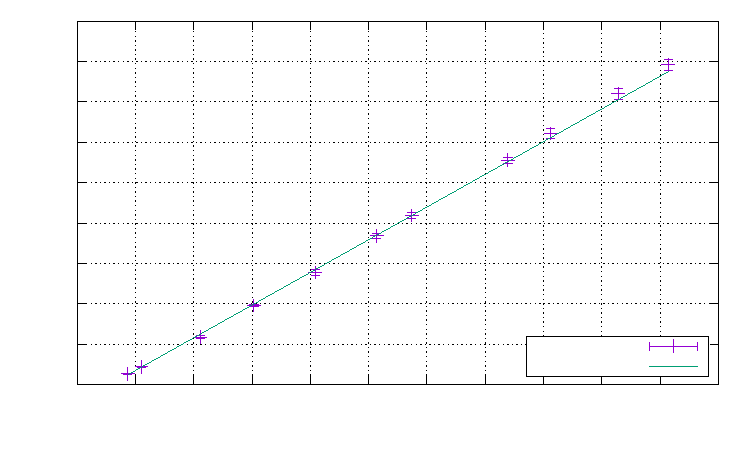
\includegraphics[width={360.00bp},height={216.00bp}]{idc}}%
    \gplfronttext
  \end{picture}%
\endgroup
}
	\caption{Stromabhängigkeit mit $\overline{\delta i^2}=\frac{V_{\text{meter}}\SI{10}{V}}{(100G_2R_f)^2}$ und $i_{\text{dc}}=-\frac{V_{\text{monitor}}}{R_f}$} \label{fig:abhängig_idc}
\end{figure}
\begin{table}[t]
	\centering
	\begin{tabular}{cc}
		\textbf{Parameter} & {\textbf{Wert(Fehler)}}    \\
		\hline
		m                  & \SI{4.049 \pm 0.038e-14}{} \\
		b                  & \SI{2.690 \pm 0.087e-19}{} \\
	\end{tabular}
	\caption{Stromabhängigkeit modelliert mit $\overline{\delta i^2}(i_{\text{dc}})=m\cdot i_{\text{dc}}+b$} \label{tab:abhängig_idc_parameter}
\end{table}

\subsubsection{Abhängigkeit $\Delta f_\text{eff}$}
Für $i_\text{dc}=\text{const.}$ wurde durch Variation der Bandbreite die Weißheit des Rauschens überprüft.
Die Weißheit gibt an, wie sich das Rauschen bei unterschiedlichen Frequenzen verhält.
Es ist weiß, wenn es frequenzunabhängig ist.
$\overline{\Delta i^2}$ ist gegen $\Delta f_{\text{eff}}$ in Abb.\ (\ref{fig:abhängig_f}) aufgetragen.
Die Parameter für den Fit sind in Tab.\ (\ref{tab:abhängig_f_parameter}) eingetragen. %TODO chi² oder auch nur guide?
Es ist zu erkennen, dass der Rauschstrom linear mit der Frequenz des Tiefpasses steigt.

\begin{figure}[t]
	\centering
	\resizebox{.5\textwidth}{!}{% GNUPLOT: LaTeX picture with Postscript
\begingroup
  \makeatletter
  \providecommand\color[2][]{%
    \GenericError{(gnuplot) \space\space\space\@spaces}{%
      Package color not loaded in conjunction with
      terminal option `colourtext'%
    }{See the gnuplot documentation for explanation.%
    }{Either use 'blacktext' in gnuplot or load the package
      color.sty in LaTeX.}%
    \renewcommand\color[2][]{}%
  }%
  \providecommand\includegraphics[2][]{%
    \GenericError{(gnuplot) \space\space\space\@spaces}{%
      Package graphicx or graphics not loaded%
    }{See the gnuplot documentation for explanation.%
    }{The gnuplot epslatex terminal needs graphicx.sty or graphics.sty.}%
    \renewcommand\includegraphics[2][]{}%
  }%
  \providecommand\rotatebox[2]{#2}%
  \@ifundefined{ifGPcolor}{%
    \newif\ifGPcolor
    \GPcolortrue
  }{}%
  \@ifundefined{ifGPblacktext}{%
    \newif\ifGPblacktext
    \GPblacktexttrue
  }{}%
  % define a \g@addto@macro without @ in the name:
  \let\gplgaddtomacro\g@addto@macro
  % define empty templates for all commands taking text:
  \gdef\gplbacktext{}%
  \gdef\gplfronttext{}%
  \makeatother
  \ifGPblacktext
    % no textcolor at all
    \def\colorrgb#1{}%
    \def\colorgray#1{}%
  \else
    % gray or color?
    \ifGPcolor
      \def\colorrgb#1{\color[rgb]{#1}}%
      \def\colorgray#1{\color[gray]{#1}}%
      \expandafter\def\csname LTw\endcsname{\color{white}}%
      \expandafter\def\csname LTb\endcsname{\color{black}}%
      \expandafter\def\csname LTa\endcsname{\color{black}}%
      \expandafter\def\csname LT0\endcsname{\color[rgb]{1,0,0}}%
      \expandafter\def\csname LT1\endcsname{\color[rgb]{0,1,0}}%
      \expandafter\def\csname LT2\endcsname{\color[rgb]{0,0,1}}%
      \expandafter\def\csname LT3\endcsname{\color[rgb]{1,0,1}}%
      \expandafter\def\csname LT4\endcsname{\color[rgb]{0,1,1}}%
      \expandafter\def\csname LT5\endcsname{\color[rgb]{1,1,0}}%
      \expandafter\def\csname LT6\endcsname{\color[rgb]{0,0,0}}%
      \expandafter\def\csname LT7\endcsname{\color[rgb]{1,0.3,0}}%
      \expandafter\def\csname LT8\endcsname{\color[rgb]{0.5,0.5,0.5}}%
    \else
      % gray
      \def\colorrgb#1{\color{black}}%
      \def\colorgray#1{\color[gray]{#1}}%
      \expandafter\def\csname LTw\endcsname{\color{white}}%
      \expandafter\def\csname LTb\endcsname{\color{black}}%
      \expandafter\def\csname LTa\endcsname{\color{black}}%
      \expandafter\def\csname LT0\endcsname{\color{black}}%
      \expandafter\def\csname LT1\endcsname{\color{black}}%
      \expandafter\def\csname LT2\endcsname{\color{black}}%
      \expandafter\def\csname LT3\endcsname{\color{black}}%
      \expandafter\def\csname LT4\endcsname{\color{black}}%
      \expandafter\def\csname LT5\endcsname{\color{black}}%
      \expandafter\def\csname LT6\endcsname{\color{black}}%
      \expandafter\def\csname LT7\endcsname{\color{black}}%
      \expandafter\def\csname LT8\endcsname{\color{black}}%
    \fi
  \fi
    \setlength{\unitlength}{0.0500bp}%
    \ifx\gptboxheight\undefined%
      \newlength{\gptboxheight}%
      \newlength{\gptboxwidth}%
      \newsavebox{\gptboxtext}%
    \fi%
    \setlength{\fboxrule}{0.5pt}%
    \setlength{\fboxsep}{1pt}%
    \definecolor{tbcol}{rgb}{1,1,1}%
\begin{picture}(7200.00,4320.00)%
    \gplgaddtomacro\gplbacktext{%
      \csname LTb\endcsname%%
      \put(829,619){\makebox(0,0)[r]{\strut{}$0.001$}}%
      \csname LTb\endcsname%%
      \put(829,1491){\makebox(0,0)[r]{\strut{}$0.01$}}%
      \csname LTb\endcsname%%
      \put(829,2362){\makebox(0,0)[r]{\strut{}$0.1$}}%
      \csname LTb\endcsname%%
      \put(829,3234){\makebox(0,0)[r]{\strut{}$1$}}%
      \csname LTb\endcsname%%
      \put(829,4106){\makebox(0,0)[r]{\strut{}$10$}}%
      \csname LTb\endcsname%%
      \put(927,425){\makebox(0,0){\strut{}$0.1$}}%
      \csname LTb\endcsname%%
      \put(2417,425){\makebox(0,0){\strut{}$1$}}%
      \csname LTb\endcsname%%
      \put(3907,425){\makebox(0,0){\strut{}$10$}}%
      \csname LTb\endcsname%%
      \put(5396,425){\makebox(0,0){\strut{}$100$}}%
      \csname LTb\endcsname%%
      \put(6886,425){\makebox(0,0){\strut{}$1000$}}%
    }%
    \gplgaddtomacro\gplfronttext{%
      \csname LTb\endcsname%%
      \put(170,2362){\rotatebox{-270}{\makebox(0,0){\strut{}$\overline{\delta i^2}/\SI{}{\nano V^2}$}}}%
      \csname LTb\endcsname%%
      \put(3906,135){\makebox(0,0){\strut{}$\Delta f_{\text{eff}}/\SI{}{\kilo Hz}$}}%
      \csname LTb\endcsname%%
      \put(6123,986){\makebox(0,0)[r]{\strut{}Daten}}%
      \csname LTb\endcsname%%
      \put(6123,793){\makebox(0,0)[r]{\strut{}Anpassung}}%
    }%
    \gplbacktext
    \put(0,0){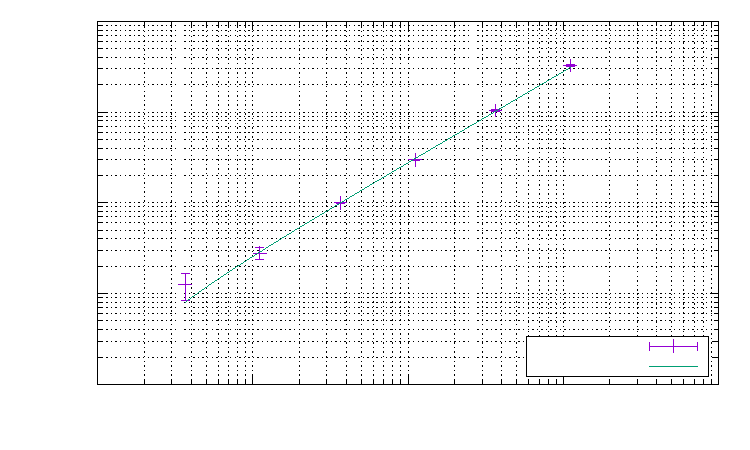
\includegraphics[width={360.00bp},height={216.00bp}]{shot_freq}}%
    \gplfronttext
  \end{picture}%
\endgroup
}
	\caption{Frequenzabhängigkeit mit $\overline{\delta i^2}=\frac{V_{\text{meter}}\SI{10}{V}}{(100G_2R_f)^2}$ und $\Delta f_{\text{eff}}=\frac{f_l\pi}{2^{3/2}}$} \label{fig:abhängig_f}
\end{figure}
\begin{table}[t]
	\centering
	\begin{tabular}{cc}
		\textbf{Parameter} & {\textbf{Wert(Fehler)}}    \\
		\hline
		m                  & \SI{2.784 \pm 0.056e-23}{} \\
		b                  & \SI{-2.2 \pm 3.0e-21}{}    \\
	\end{tabular}
	\caption{Frequenzabhängigkeit modelliert mit $\overline{\delta i^2}(f)=m\cdot f+b$} \label{tab:abhängig_f_parameter}
\end{table}

\subsubsection{Elementarladung}

\begin{table}[t]
	\centering
	\begin{tabular}{cc}
		\textbf{Parameter} & {\textbf{Wert(Fehler)}} \\
		\hline
		$f_l$              & \SI{10104 \pm 56}{}     \\
		$f_h$              & \SI{100.50 \pm 0.17}{}  \\
	\end{tabular}
	\caption{Frequenzabhängigkeit modelliert mit $G_\text{LP}(f)=\left[1+(f/f_l)^4\right]^{-1/2}$ und $G_\text{HP}(f)=(f/f_h)^2\left[1+(f/f_h)^4\right]^{-1/2}$} \label{tab:parameter}
\end{table}
%TODO was ist die tabelle?


\bibliography{refs}

\end{document}
